\documentclass[11pt,a4paper]{report}
\usepackage[textwidth=37em,vmargin=30mm]{geometry}
\usepackage{calc,xunicode,amsmath,amssymb,paralist,enumitem,tabu,booktabs,datetime2,xeCJK,xeCJKfntef,listings}
\usepackage{tocloft,fancyhdr,tcolorbox,xcolor,graphicx,eso-pic,xltxtra,xelatexemoji}

\newcommand{\envyear}[0]{2025}
\newcommand{\envdatestr}[0]{2025-06-06}
\newcommand{\envfinaldir}[0]{webdb/2025/20250606/final}

\usepackage[hidelinks]{hyperref}
\hypersetup{
    colorlinks=false,
    pdfpagemode=FullScreen,
    pdftitle={Web Digest - \envdatestr}
}

\setlength{\cftbeforechapskip}{10pt}
\renewcommand{\cftchapfont}{\rmfamily\bfseries\large\raggedright}
\setlength{\cftbeforesecskip}{2pt}
\renewcommand{\cftsecfont}{\sffamily\small\raggedright}

\setdefaultleftmargin{2em}{2em}{1em}{1em}{1em}{1em}

\usepackage{xeCJK,xeCJKfntef}
\xeCJKsetup{PunctStyle=plain,RubberPunctSkip=false,CJKglue=\strut\hskip 0pt plus 0.1em minus 0.05em,CJKecglue=\strut\hskip 0.22em plus 0.2em}
\XeTeXlinebreaklocale "zh"
\XeTeXlinebreakskip = 0pt


\setmainfont{Brygada 1918}
\setromanfont{Brygada 1918}
\setsansfont{IBM Plex Sans}
\setmonofont{JetBrains Mono NL}
\setCJKmainfont{Noto Serif CJK SC}
\setCJKromanfont{Noto Serif CJK SC}
\setCJKsansfont{Noto Sans CJK SC}
\setCJKmonofont{Noto Sans CJK SC}

\setlength{\parindent}{0pt}
\setlength{\parskip}{8pt}
\linespread{1.15}

\lstset{
	basicstyle=\ttfamily\footnotesize,
	numbersep=5pt,
	backgroundcolor=\color{black!5},
	showspaces=false,
	showstringspaces=false,
	showtabs=false,
	tabsize=2,
	captionpos=b,
	breaklines=true,
	breakatwhitespace=true,
	breakautoindent=true,
	linewidth=\textwidth
}






\newcommand{\coverpic}[2]{
    % argv: itemurl, authorname
    Cover photo by #2~~(\href{#1}{#1})
}
\newcommand{\makeheader}[0]{
    \begin{titlepage}
        % \newgeometry{hmargin=15mm,tmargin=21mm,bmargin=12mm}
        \begin{center}
            
            \rmfamily\scshape
            \fontspec{BaskervilleF}
            \fontspec{Old Standard}
            \fontsize{59pt}{70pt}\selectfont
            WEB\hfill DIGEST
            
            \vfill
            % \vskip 30pt
            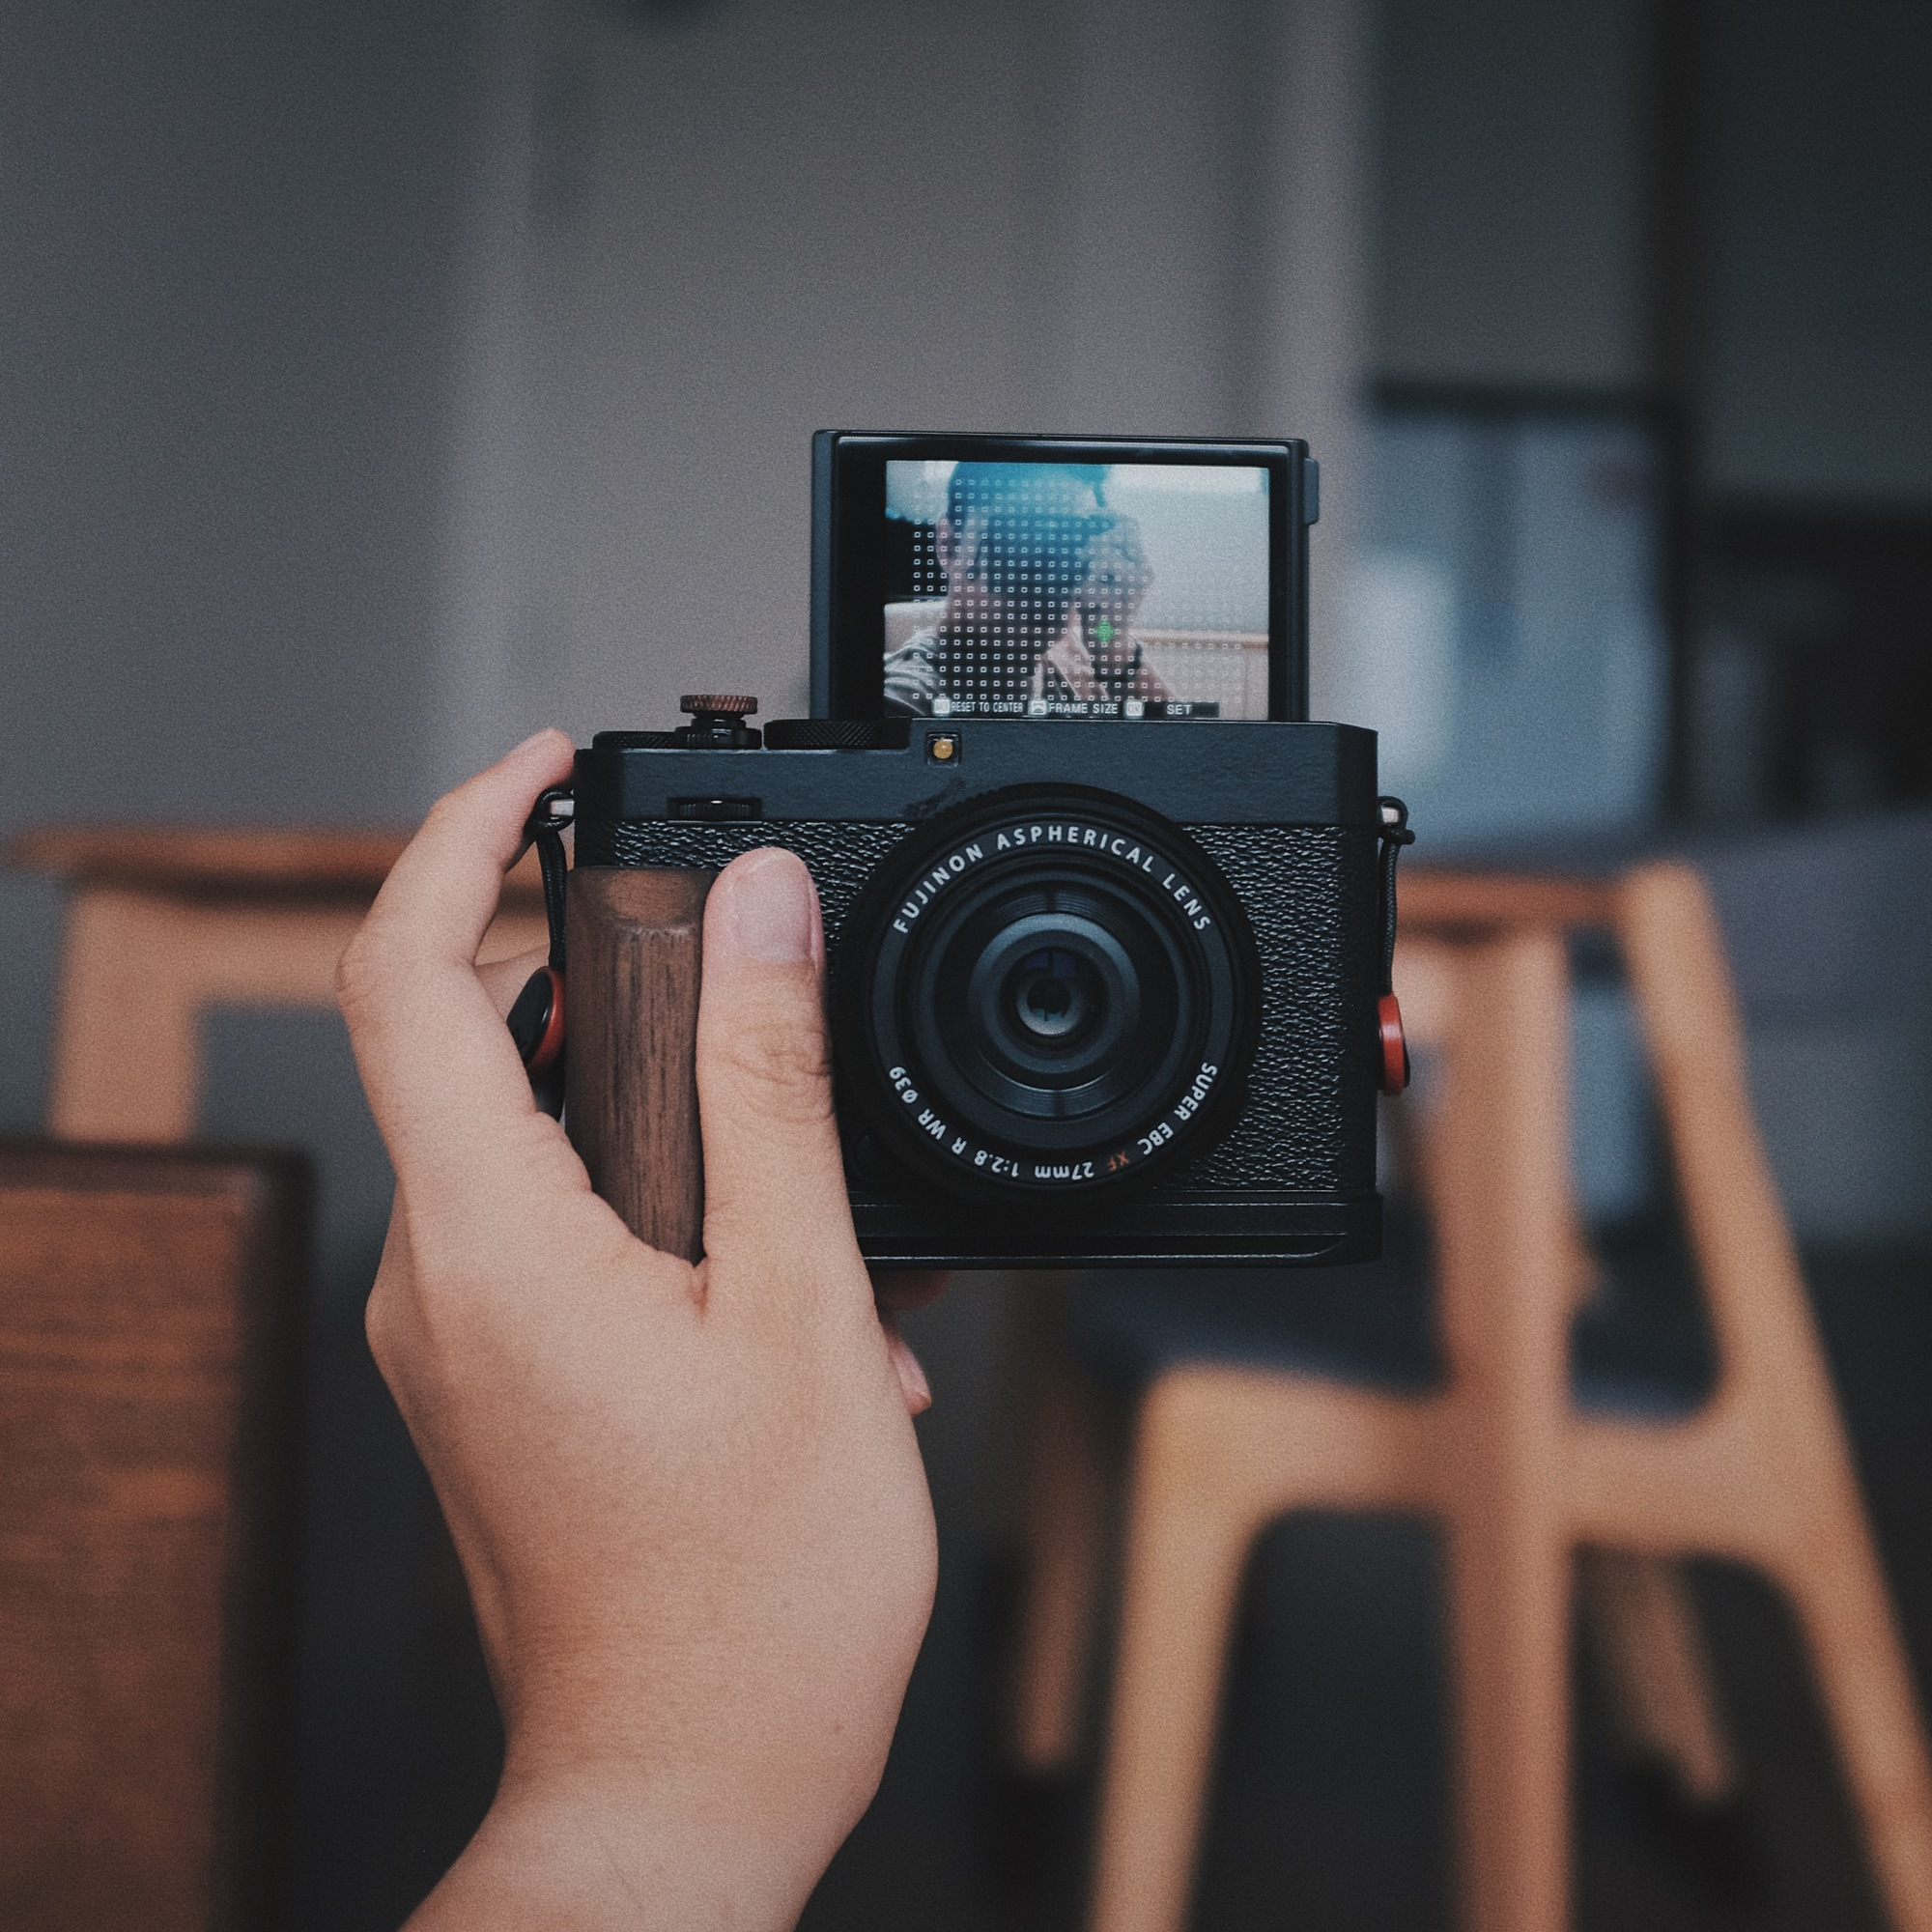
\includegraphics[width=\linewidth]{\envfinaldir/coverpic-prod.jpg}\par
            % \vskip 30pt
            \vfill

            \normalsize\rmfamily\scshape
            \copyright{} The Web Digest Project \hfill\large \envdatestr
        \end{center}
    \end{titlepage}
    % \restoregeometry
}
\newcommand{\simplehref}[1]{%
    \textcolor{blue!80!green}{\href{#1}{#1}}%
}
\renewcommand{\contentsname}{\center\Huge\sffamily\bfseries Contents\par\vskip 20pt}
\newcounter{ipartcounter}
\setcounter{ipartcounter}{0}
\newcommand{\ipart}[1]{
    % \vskip 20pt
    \clearpage
    \stepcounter{ipartcounter}
    \phantomsection
    \addcontentsline{toc}{chapter}{#1}
    % \begin{center}
    %     \Huge
    %     \sffamily\bfseries
    %     #1
    % \end{center}
    % \vskip 20pt plus 7pt
}
\newcounter{ichaptercounter}
\setcounter{ichaptercounter}{0}
\newcommand{\ichapter}[1]{
    % \vskip 20pt
    \clearpage
    \stepcounter{ichaptercounter}
    \phantomsection
    \addcontentsline{toc}{section}{\numberline{\arabic{ichaptercounter}}#1}
    \begin{center}
        \Huge
        \sffamily\bfseries
        #1
    \end{center}
    \vskip 20pt plus 7pt
}
\newcommand{\entrytitlefont}[1]{\subsection*{\raggedright\Large\sffamily\bfseries#1}}
\newcommand{\entryitemGeneric}[2]{
    % argv: title, url
    \parbox{\linewidth}{
        \entrytitlefont{#1}\par\vskip 5pt
        \footnotesize\ttfamily\mdseries
        \simplehref{#2}
    }\vskip 11pt plus 11pt minus 1pt
}
\newcommand{\entryitemGithub}[3]{
    % argv: title, url, desc
    \parbox{\linewidth}{
        \entrytitlefont{#1}\par\vskip 5pt
        \footnotesize\ttfamily\mdseries
        \simplehref{#2}\par\vskip 5pt
        \small\rmfamily\mdseries#3
    }\vskip 11pt plus 11pt minus 1pt
}
\newcommand{\entryitemAp}[3]{
    % argv: title, url, desc
    \parbox{\linewidth}{
        \entrytitlefont{#1}\par\vskip 5pt
        \footnotesize\ttfamily\mdseries
        \simplehref{#2}\par\vskip 5pt
        \small\rmfamily\mdseries#3
    }\vskip 11pt plus 11pt minus 1pt
}
\newcommand{\entryitemHackernews}[3]{
    % argv: title, hnurl, rawurl
    % \parbox{\linewidth}{
    %     \entrytitlefont{#1}\par\vskip 5pt
    %     \footnotesize\ttfamily\mdseries
    %     \simplehref{#3}\par
    %     \textcolor{black!50}{\href{#2}{#2}}
    % }\vskip 11pt plus 11pt minus 1pt
    \begin{minipage}{\linewidth}
            \entrytitlefont{#1}\par\vskip 5pt
            \footnotesize\ttfamily\mdseries
            \simplehref{#3}\par
            \textcolor{black!50}{\href{#2}{#2}}
    \end{minipage}\par\vskip 11pt plus 11pt minus 1pt
}







\begin{document}

\makeheader

\tableofcontents\clearpage




\ipart{Developers}
\ichapter{Hacker News}
\entryitemTwoLinks{Eleven v3}{https://news.ycombinator.com/item?id=44194521}{https://elevenlabs.io/v3}

\entryitemTwoLinks{Show HN: ClickStack – Open-source Datadog alternative by ClickHouse and HyperDX}{https://news.ycombinator.com/item?id=44194082}{https://github.com/hyperdxio/hyperdx}

\entryitemTwoLinks{Gemini-2.5-pro-preview-06-05}{https://news.ycombinator.com/item?id=44193328}{https://deepmind.google/models/gemini/pro/}

\entryitemTwoLinks{Google restricts Android sideloading}{https://news.ycombinator.com/item?id=44193198}{https://puri.sm/posts/google-restricts-android-sideloading-what-it-means-for-user-autonomy-and-the-future-of-mobile-freedom/}

\entryitemTwoLinks{Rare black iceberg spotted off Labrador coast could be 100k years old}{https://news.ycombinator.com/item?id=44193120}{https://www.cbc.ca/news/canada/newfoundland-labrador/black-iceberg-labrador-coast-1.7551078}

\entryitemTwoLinks{I think I'm done thinking about GenAI for now}{https://news.ycombinator.com/item?id=44193018}{https://blog.glyph.im/2025/06/i-think-im-done-thinking-about-genai-for-now.html}

\entryitemTwoLinks{Seven Days at the Bin Store}{https://news.ycombinator.com/item?id=44192995}{https://defector.com/seven-days-at-the-bin-store}

\entryitemTwoLinks{The impossible predicament of the death newts}{https://news.ycombinator.com/item?id=44191620}{https://crookedtimber.org/2025/06/05/occasional-paper-the-impossible-predicament-of-the-death-newts/}

\entryitemTwoLinks{Twitter's new encrypted DMs aren't better than the old ones}{https://news.ycombinator.com/item?id=44191591}{https://mjg59.dreamwidth.org/71646.html}

\entryitemTwoLinks{Apple Notes Will Gain Markdown Export at WWDC, and, I Have Thoughts}{https://news.ycombinator.com/item?id=44191558}{https://daringfireball.net/linked/2025/06/04/apple-notes-markdown}

\entryitemTwoLinks{10 Years of Betting on Rust}{https://news.ycombinator.com/item?id=44190190}{https://tably.com/tably/10-years-of-betting-on-rust}

\entryitemTwoLinks{From tokens to thoughts: How LLMs and humans trade compression for meaning}{https://news.ycombinator.com/item?id=44189426}{https://arxiv.org/abs/2505.17117}

\entryitemTwoLinks{Air Lab – A portable and open air quality measuring device}{https://news.ycombinator.com/item?id=44189329}{https://networkedartifacts.com/airlab/simulator}

\entryitemTwoLinks{End of an Era: Landsat 7 Decommissioned After 25 Years of Earth Observation}{https://news.ycombinator.com/item?id=44188248}{https://www.usgs.gov/news/national-news-release/end-era-landsat-7-decommissioned-after-25-years-earth-observation}

\entryitemTwoLinks{Old payphones get new life, thanks to Vermont engineer}{https://news.ycombinator.com/item?id=44188204}{https://www.core77.com/posts/137183/Engineer-Fixes-and-Re-Installs-Old-Payphones-Provides-Free-Calls-to-the-Public}

\entryitemTwoLinks{Show HN: I made a 3D SVG Renderer that projects textures without rasterization}{https://news.ycombinator.com/item?id=44187645}{https://seve.blog/p/i-made-a-3d-svg-renderer-that-projects}

\entryitemTwoLinks{Tesla seeks to guard crash data from public disclosure}{https://news.ycombinator.com/item?id=44186780}{https://www.reuters.com/legal/government/musks-tesla-seeks-guard-crash-data-public-disclosure-2025-06-04/}

\entryitemTwoLinks{A Spiral Structure in the Inner Oort Cloud}{https://news.ycombinator.com/item?id=44186660}{https://iopscience.iop.org/article/10.3847/1538-4357/adbf9b}

\entryitemTwoLinks{parrot.live}{https://news.ycombinator.com/item?id=44186536}{https://github.com/hugomd/parrot.live}

\entryitemTwoLinks{LLMs and Elixir: Windfall or Deathblow?}{https://news.ycombinator.com/item?id=44186496}{https://www.zachdaniel.dev/p/llms-and-elixir-windfall-or-deathblow}\ichapter{Dribbble}
\entryitemGeneric{\hskip 0pt{}Aquasan}{https://dribbble.com/shots/26100535-Aquasan}

\entryitemGeneric{\hskip 0pt{}Eagle}{https://dribbble.com/shots/26099428-Eagle}

\entryitemGeneric{\hskip 0pt{}Mnp Technologies - Logo Design}{https://dribbble.com/shots/26092034-Mnp-Technologies-Logo-Design}

\entryitemGeneric{\hskip 0pt{}Singular Logo Concept (Unused)}{https://dribbble.com/shots/26091755-Singular-Logo-Concept-Unused}

\entryitemGeneric{\hskip 0pt{}Cre8tera // Website}{https://dribbble.com/shots/26091009-Cre8tera-Website}

\entryitemGeneric{\hskip 0pt{}Cool Pool Logo Design - Letter C Monogram}{https://dribbble.com/shots/26091401-Cool-Pool-Logo-Design-Letter-C-Monogram}

\entryitemGeneric{\hskip 0pt{}Gorilla + Bar Chart Logo}{https://dribbble.com/shots/26092670-Gorilla-Bar-Chart-Logo}

\entryitemGeneric{\hskip 0pt{}zeero logo design}{https://dribbble.com/shots/26087342-zeero-logo-design}

\entryitemGeneric{\hskip 0pt{}Create email inbox composition}{https://dribbble.com/shots/26083118-Create-email-inbox-composition}

\entryitemGeneric{\hskip 0pt{}Shori Brand}{https://dribbble.com/shots/26088139-Shori-Brand}

\entryitemGeneric{\hskip 0pt{}Roaring Bear}{https://dribbble.com/shots/26087788-Roaring-Bear}

\entryitemGeneric{\hskip 0pt{}Eagle}{https://dribbble.com/shots/26085536-Eagle}

\entryitemGeneric{\hskip 0pt{}Hand-drawn illustration pack}{https://dribbble.com/shots/26084735-Hand-drawn-illustration-pack}

\entryitemGeneric{\hskip 0pt{}Dog Mascot Various Poses}{https://dribbble.com/shots/26087977-Dog-Mascot-Various-Poses}

\entryitemGeneric{\hskip 0pt{}Branding Concept for Europe}{https://dribbble.com/shots/26087652-Branding-Concept-for-Europe}

\entryitemGeneric{\hskip 0pt{}B2B Dashboard \& Web App UI UX Design for Carbon Solutions}{https://dribbble.com/shots/26076624-B2B-Dashboard-Web-App-UI-UX-Design-for-Carbon-Solutions}

\entryitemGeneric{\hskip 0pt{}Patriot Logo Design (Unused for Sale)}{https://dribbble.com/shots/26081047-Patriot-Logo-Design-Unused-for-Sale}

\entryitemGeneric{\hskip 0pt{}Heliopoint}{https://dribbble.com/shots/26081987-Heliopoint}

\entryitemGeneric{\hskip 0pt{}Apple}{https://dribbble.com/shots/26084067-Apple}

\entryitemGeneric{\hskip 0pt{}Illustration}{https://dribbble.com/shots/26083223-Illustration}

\entryitemGeneric{\hskip 0pt{}Europe Logo Animation}{https://dribbble.com/shots/26082596-Europe-Logo-Animation}

\entryitemGeneric{\hskip 0pt{}Arc Logo}{https://dribbble.com/shots/26083648-Arc-Logo}

\entryitemGeneric{\hskip 0pt{}Heyo Turns 2!}{https://dribbble.com/shots/26078572-Heyo-Turns-2}

\entryitemGeneric{\hskip 0pt{}Fox Brand Mascot}{https://dribbble.com/shots/26077954-Fox-Brand-Mascot}


\ipart{Developers~~~~(zh-Hans)}
\ichapter{Solidot}
\entryitemGeneric{\hskip 0pt{}特斯拉汽车销量在欧洲继续下滑}{https://www.solidot.org/story?sid=81480}

\entryitemGeneric{\hskip 0pt{}Wendelstein 7-X 仿星器创下可控核聚变新纪录}{https://www.solidot.org/story?sid=81479}

\entryitemGeneric{\hskip 0pt{}Google Chrome 撤销对中华电信和 Netlock CA 的信任}{https://www.solidot.org/story?sid=81478}

\entryitemGeneric{\hskip 0pt{}随着 Windows 10 即将终止支持,KDE 项目试图吸引微软用户}{https://www.solidot.org/story?sid=81477}

\entryitemGeneric{\hskip 0pt{}草帽星系可能经历过星系合并}{https://www.solidot.org/story?sid=81476}

\entryitemGeneric{\hskip 0pt{}科学家发现一颗位于宜居带的超级地球}{https://www.solidot.org/story?sid=81475}

\entryitemGeneric{\hskip 0pt{}蓬勃发展的克隆动物生意}{https://www.solidot.org/story?sid=81474}

\entryitemGeneric{\hskip 0pt{}Reddit 起诉 Anthropic 违反合同和不公平竞争}{https://www.solidot.org/story?sid=81473}

\entryitemGeneric{\hskip 0pt{}韦伯发现已知最遥远的星系}{https://www.solidot.org/story?sid=81472}

\entryitemGeneric{\hskip 0pt{}Meta Android 应用停止使用移动端口跟踪技术}{https://www.solidot.org/story?sid=81471}

\entryitemGeneric{\hskip 0pt{}为遵守欧盟法律微软给予欧洲用户对 Windows 更多的控制权}{https://www.solidot.org/story?sid=81470}

\entryitemGeneric{\hskip 0pt{}微软测试给记事本添加 Markdown}{https://www.solidot.org/story?sid=81469}

\entryitemGeneric{\hskip 0pt{}科学家确认 2023 年发生的神秘震动源自格陵兰岛海啸}{https://www.solidot.org/story?sid=81468}

\entryitemGeneric{\hskip 0pt{}特朗普政府的 2026 年预算将为商业火星探索拨款逾 10 亿美元}{https://www.solidot.org/story?sid=81467}

\entryitemGeneric{\hskip 0pt{}日本 2024 年新生儿数首次跌破 70 万}{https://www.solidot.org/story?sid=81466}

\entryitemGeneric{\hskip 0pt{}AI 创业公司被发现其聊天机器人是 700 名印度员工}{https://www.solidot.org/story?sid=81465}

\entryitemGeneric{\hskip 0pt{}OpenAI 董事会短暂解雇 CEO Sam Altman 的故事被搬上银幕}{https://www.solidot.org/story?sid=81464}

\entryitemGeneric{\hskip 0pt{}印度便利店应用 KiranaPro 被删库}{https://www.solidot.org/story?sid=81460}

\entryitemGeneric{\hskip 0pt{}研究确定背包问题计算复杂性下限}{https://www.solidot.org/story?sid=81459}

\entryitemGeneric{\hskip 0pt{}神秘告密者公开勒索软件组织关键成员身份}{https://www.solidot.org/story?sid=81458}\ichapter{V2EX}
\entryitemGeneric{\hskip 0pt{}[分享创造] LynxProxy 代理抓包工具 v0.2.0 发布,支持规则捕获}{https://www.v2ex.com/t/1136702}

\entryitemGeneric{\hskip 0pt{}[程序员] Claude Code 現在只需要 20 美元了}{https://www.v2ex.com/t/1136701}

\entryitemGeneric{\hskip 0pt{}[Android] 618, 求推荐款可折叠,可刷机的国产(国际版)安卓机?}{https://www.v2ex.com/t/1136700}

\entryitemGeneric{\hskip 0pt{}[问与答] 求教求教 cursor 的用法和问题,}{https://www.v2ex.com/t/1136698}

\entryitemGeneric{\hskip 0pt{}[推广] vibe 了个 chrome 插件发现网站}{https://www.v2ex.com/t/1136697}

\entryitemGeneric{\hskip 0pt{}[生活] 安卓 TV 上有什么好用的 emby 客户端吗}{https://www.v2ex.com/t/1136694}

\entryitemGeneric{\hskip 0pt{}[问与答] 不止一次发现 chatgpt 在耗电}{https://www.v2ex.com/t/1136693}

\entryitemGeneric{\hskip 0pt{}[问与答] 第一次养柴犬,冠能幼犬粮 vs 皇家柴犬专用粮,怎么选更合适?}{https://www.v2ex.com/t/1136692}

\entryitemGeneric{\hskip 0pt{}[问与答] 无房无车 50W 彩礼算高额吗}{https://www.v2ex.com/t/1136691}

\entryitemGeneric{\hskip 0pt{}[分享发现] 新的 Hugo 主题 Hugo Narrow}{https://www.v2ex.com/t/1136690}

\entryitemGeneric{\hskip 0pt{}[微信] 关于微信的 livekit 锁屏不能正常显示弹窗的问题及解决办法}{https://www.v2ex.com/t/1136689}

\entryitemGeneric{\hskip 0pt{}[酷工作] [招聘帖] 全职远程技术岗🌍| AI+Crypto 华人创业团队融资已到位] 6 月新职位: Sr.Full-Stack Engineer /Sr.Data/Sr .Staff AI/企业直聘}{https://www.v2ex.com/t/1136687}

\entryitemGeneric{\hskip 0pt{}[Go 编程语言] Go 团队的错误处理决定:背离工程实践的官僚作风?(本文经 LLM 润色)}{https://www.v2ex.com/t/1136685}

\entryitemGeneric{\hskip 0pt{}[YouTube] 很奇怪,油管上的很多视频,为何大部分都是 SDR 显示技术,而非 HDR 显示技术?}{https://www.v2ex.com/t/1136684}

\entryitemGeneric{\hskip 0pt{}[问与答] 现在用的北京移动 9 元套餐,有没有便宜的 1~ 2G 流量包呢?}{https://www.v2ex.com/t/1136681}

\entryitemGeneric{\hskip 0pt{}[分享创造] 我用 AI 写了一个找不同游戏网站,欢迎大家体验。}{https://www.v2ex.com/t/1136680}

\entryitemGeneric{\hskip 0pt{}[Apple] 家里有一台旧的 mac mini 2018 i7 64g 还可以发挥什么剩余价值呢?}{https://www.v2ex.com/t/1136679}

\entryitemGeneric{\hskip 0pt{}[macOS] macbook air m3 睡眠是烫的,开机是凉的}{https://www.v2ex.com/t/1136678}

\entryitemGeneric{\hskip 0pt{}[Nintendo Switch] 咨询现在注册哪个区的服?刚入 switch2}{https://www.v2ex.com/t/1136677}

\entryitemGeneric{\hskip 0pt{}[问与答] 有没有办法允许剪切但是不允许删除?}{https://www.v2ex.com/t/1136676}

\entryitemGeneric{\hskip 0pt{}[酷工作] [远程] 招聘 QA 测试工程师/前端/后端/iOS 开发工程师 [GiggleAcademy]}{https://www.v2ex.com/t/1136674}

\entryitemGeneric{\hskip 0pt{}[分享创造] 🎹 写了个键盘十字键导航 js 库,原理简单、引入开发简单、用户体验更简单}{https://www.v2ex.com/t/1136671}

\entryitemGeneric{\hskip 0pt{}[问与答] 关于 qq 邮箱网页版:为什么我已经登陆了还在显示拉取二维码,还有上报 clc 是什么}{https://www.v2ex.com/t/1136669}

\entryitemGeneric{\hskip 0pt{}[生活] 约 AI Coding 从业者 CoffeeChat}{https://www.v2ex.com/t/1136667}

\entryitemGeneric{\hskip 0pt{}[上海] 十二生肖觉醒!}{https://www.v2ex.com/t/1136666}

\entryitemGeneric{\hskip 0pt{}[问与答] ``SFM''想访问其他 App 的数据。}{https://www.v2ex.com/t/1136664}

\entryitemGeneric{\hskip 0pt{}[程序员] 关于 Minio 后台 ui 页面的显示}{https://www.v2ex.com/t/1136663}

\entryitemGeneric{\hskip 0pt{}[问与答] 云服务提供商是否有义务出售未被 BAN 的全新服务器和全新域名?}{https://www.v2ex.com/t/1136662}

\entryitemGeneric{\hskip 0pt{}[职场话题] 为什么面试问题(暑期 Java 后端实习)都回答上来了还是被秒挂了呢}{https://www.v2ex.com/t/1136660}

\entryitemGeneric{\hskip 0pt{}[程序员] 各位开源软件作者们是否可以考虑用 AI 把文档提升一下?}{https://www.v2ex.com/t/1136658}

\entryitemGeneric{\hskip 0pt{}[Google] Gemini 2.5 Pro 的联网搜索分析能力变弱了,难道转向了 NotebookLM}{https://www.v2ex.com/t/1136657}

\entryitemGeneric{\hskip 0pt{}[程序员] 支付宝付款成功页面可以去广告吗}{https://www.v2ex.com/t/1136656}

\entryitemGeneric{\hskip 0pt{}[分享发现] 离谱!联通私自变更用户套餐}{https://www.v2ex.com/t/1136655}

\entryitemGeneric{\hskip 0pt{}[问与答] 微信输入法磁盘写入字节很多,正常吗 https://imgur.com/AYKjmQY}{https://www.v2ex.com/t/1136654}

\entryitemGeneric{\hskip 0pt{}[职场话题] 被裁了,有点迷茫,求点建议和指点}{https://www.v2ex.com/t/1136653}

\entryitemGeneric{\hskip 0pt{}[投资] 活钱 02 | 4 步学会安全理财,远离诈骗陷阱}{https://www.v2ex.com/t/1136652}

\entryitemGeneric{\hskip 0pt{}[分享创造] 上线了一个油猴脚本,复刻了 macOS 上 PopClip 中的 ``Large Type'' 功能}{https://www.v2ex.com/t/1136651}

\entryitemGeneric{\hskip 0pt{}[VXNA] 申请收录个人博客:上岸的鱼}{https://www.v2ex.com/t/1136650}

\entryitemGeneric{\hskip 0pt{}[分享发现] 飞牛私有云 fnOS 系统 影视应用更新 V0.8.46 2025/6/5}{https://www.v2ex.com/t/1136649}

\entryitemGeneric{\hskip 0pt{}[云计算] 目前大家公司是怎么用公有云的?}{https://www.v2ex.com/t/1136648}

\entryitemGeneric{\hskip 0pt{}[Android] 国行三星和国际三星手机 硬件,软件差别大吗?在硬件相同的情况下可互刷?}{https://www.v2ex.com/t/1136647}

\entryitemGeneric{\hskip 0pt{}[Go 编程语言] 来个会 GO 的,付费帮忙处理个问题}{https://www.v2ex.com/t/1136646}

\entryitemGeneric{\hskip 0pt{}[分享创造] [持续免费体验中] www.chatnova.im ChatNova V1.1.0 版本速览! 6 大升级点直击效率💥}{https://www.v2ex.com/t/1136642}

\entryitemGeneric{\hskip 0pt{}[生活] 个税汇算, 7 项专项扣除及高频问题,家庭夫妻二人根据税率不同巧安排,退得多!}{https://www.v2ex.com/t/1136641}

\entryitemGeneric{\hskip 0pt{}[Tesla] 车主引荐 免费选 8k 车漆}{https://www.v2ex.com/t/1136640}

\entryitemGeneric{\hskip 0pt{}[问与答] 有没有老哥通俗易懂地讲讲中枢网关和蓝牙网关有什么区别}{https://www.v2ex.com/t/1136639}

\entryitemGeneric{\hskip 0pt{}[分享创造] 为了让你通过阅读学英语,我整理了 50 个英语信息源}{https://www.v2ex.com/t/1136636}

\entryitemGeneric{\hskip 0pt{}[分享发现] 有玩银河放置奶牛的吗,这两天摸鱼玩的挺不错}{https://www.v2ex.com/t/1136635}

\entryitemGeneric{\hskip 0pt{}[程序员] 大家有没有这种批量抓取视频评论的网站或者服务,最好是按量付费}{https://www.v2ex.com/t/1136633}

\entryitemGeneric{\hskip 0pt{}[V2EX] 写了一个油猴脚本屏蔽 HDR 图片}{https://www.v2ex.com/t/1136632}


\ipart{Generic News}
\ichapter{AP News}
\entryitemWithDescription{\hskip 0pt{}FanDuel bans bettor over heckling incident with Olympic champion sprinter Gabby Thomas}{https://apnews.com/article/d226103292fdf6c019f0c71435e9745e}{}

\entryitemWithDescription{\hskip 0pt{}Ex-White House press secretary Karine Jean-Pierre left Democratic Party, publisher of her book says}{https://apnews.com/article/fbb44b9eb3bb56f6ab8ef02bd7ffa042}{}

\entryitemWithDescription{\hskip 0pt{}Dilly Dally the sea turtle returns to the ocean after flipper amputation}{https://apnews.com/article/3310f37f8901e539453c22ca40dabc00}{}

\entryitemWithDescription{\hskip 0pt{}Hegseth orders the name of gay rights activist Harvey Milk scrubbed from Navy ship}{https://apnews.com/article/d6cda5df15ee5bc066092d54c591c6f2}{}

\entryitemWithDescription{\hskip 0pt{}Reddit sues AI company Anthropic for allegedly `scraping' user comments to train chatbot Claude}{https://apnews.com/article/f5ea042beb253a3f05a091e70531692d}{}

\entryitemWithDescription{\hskip 0pt{}A long-running experiment finds a tiny particle is still acting weird}{https://apnews.com/article/cb123cd20bfd8141dbf75de62804b32b}{}

\entryitemWithDescription{\hskip 0pt{}Woman who denies mushroom murders of her in-laws accepts that she served them death caps for lunch}{https://apnews.com/article/00ea28021943fe4a56d2a3b30ad26598}{}

\entryitemWithDescription{\hskip 0pt{}What made Mount Etna's latest eruption so rare}{https://apnews.com/article/1adafac765158138817a2c4319ce1468}{}

\entryitemWithDescription{\hskip 0pt{}Northern lights could be visible again in some US states after weekend solar storms}{https://apnews.com/article/915a2364b24679c63a07066f55c53ffa}{}

\entryitemWithDescription{\hskip 0pt{}Eagles' Saquon Barkley announced as Madden NFL 26 cover athlete}{https://apnews.com/article/3b0254fa10fb8df98e91562be76d8d5c}{}

\entryitemWithDescription{\hskip 0pt{}Bills QB Josh Allen and actor Hailee Steinfeld marry in Southern California}{https://apnews.com/article/7d152f7f490a3d8ee28d6031bf02b3a0}{}

\entryitemWithDescription{\hskip 0pt{}And with that, an era ends: `Thanks for watching us. It's the NBA on TNT'}{https://apnews.com/article/8d11e74bf32e77de886add0225f108ef}{}

\entryitemWithDescription{\hskip 0pt{}The NBA Finals are set: It'll be Thunder vs. Pacers, starting Thursday night}{https://apnews.com/article/fcb0ef3120847d1d6f515fc5fe5bf04a}{}






\clearpage
\leavevmode\vfill
\footnotesize

Copyright \copyright{} 2023-2025 Neruthes and other contributors.

This document is published with CC BY-NC-ND 4.0 license.

The entries listed in this newsletter may be copyrighted by their respective creators.

This newsletter is generated by the Web Digest project.

The newsletters are also delivered via Telegram channel \CJKunderline{\href{https://t.me/webdigestchannel}{https://t.me/webdigestchannel}}.\\
RSS feed is available at \CJKunderline{\href{https://webdigest.pages.dev/rss.xml}{https://webdigest.pages.dev/rss.xml}}.

This newsletter is available in PDF at
\CJKunderline{\href{https://webdigest.pages.dev/}{https://webdigest.pages.dev/}}.

The source code being used to generate this newsletter is available at\\
\CJKunderline{\href{https://github.com/neruthes/webdigest}{https://github.com/neruthes/webdigest}}.

This newsletter is also available in
\CJKunderline{\href{http://webdigest.pages.dev/readhtml/\envyear/WebDigest-20250606.html}{HTML}} and
\CJKunderline{\href{https://github.com/neruthes/webdigest/blob/master/markdown/\envyear/WebDigest-20250606.md}{Markdown}}.


\coverpic{https://unsplash.com/photos/plants-and-decor-sit-on-a-shelf-adgKokgYMRc}{Tanya Yarosh}


\end{document}
